\documentclass[12pt, a4paper]{article}

% Essential Packages
\usepackage[utf8]{inputenc}
\usepackage[T1]{fontenc}
\usepackage{geometry}
\usepackage{titlesec}
\usepackage{hyperref}
\usepackage{graphicx}
\usepackage{natbib} % For bibliography management
\usepackage{amsmath}
\usepackage{amssymb} % Added for extra math symbols if needed
\usepackage{booktabs} % For nicer tables
\usepackage{xcolor}
\usepackage{tikz}
\usetikzlibrary{positioning, arrows.meta, fit, backgrounds, calc}

% Page Geometry
\geometry{
    left=25mm,
    right=25mm,
    top=25mm,
    bottom=25mm,
}

% Title Information
\title{\textbf{Cross-Modal Attention for Egyptian Arabic Multimodal Emotion Recognition: A Systematic Review and Research Proposal}}
\author{Nour Gaser, Mohamed Wael \\ 
\textit{Department of Computer Science} \\ 
\textit{German International University}}
\date{February 2026}

\begin{document}

\maketitle

\begin{abstract}
    \textbf{Context:} Multimodal Sentiment Analysis (MSA) has seen significant advancements in high-resource languages, yet Arabic---specifically dialectal variants like Egyptian---remains under-researched.
    \textbf{Problem:} Current baselines for Arabic multimodal datasets, such as EGY-MER, predominantly rely on ``Late Fusion'' techniques. These methods process modalities (text, audio, video) independently, often failing to capture critical inter-modal dynamics such as sarcasm or emotional inconsistency.
    \textbf{Proposal:} Cross-modal attention reached Arabic multimodal sentiment analysis during 2026, but exclusively on three-class polarity over corpora of several thousand samples. Whether that advantage survives the move to seven-class categorical emotion on a dialectal corpus an order of magnitude smaller is untested. This paper reports a systematic review of 1{,}322 retrieved records covering the field to July 2026, and proposes an experimental framework addressing that question.
    \textbf{Methodology:} A Tri-Modal Cross-Attention Network is evaluated against a re-implemented gated late-fusion baseline over identical frozen features, across three corpora selected to separate task regime, corpus scale and dialect. The design yields an interpretable result whether or not the attention mechanism proves advantageous in the low-resource emotion setting.
\end{abstract}

% ----------------------------------------------------------------------

\section{Introduction}\label{sec:intro}
The exponential growth of video content in the Arab world (e.g., YouTube, TikTok) has necessitated the development of automated systems capable of understanding human emotion beyond mere text. While English-language research has benefited from massive benchmarks like CMU-MOSI, Arabic resources have historically been scarce \citep{Haouhat2023}.

Recently, 2025 has seen the release of significant datasets such as \textbf{EGY-MER} \citep{Hussein2025} and \textbf{Ar-MuSA} \citep{Khaled2025}, which focus on dialectal Arabic (Egyptian, Saudi, and Darija). However, the baseline models established for these datasets largely rely on \textbf{Late Fusion}---a technique that concatenates feature vectors only at the final classification stage.

This review analyzes the limitations of these current baselines and establishes the theoretical justification for implementing \textbf{Cross-Modal Attention}, a method that allows the text model to dynamically ``attend'' to specific visual frames or audio segments, thereby capturing fine-grained interactions required for detecting complex emotions in Egyptian Arabic.

% ----------------------------------------------------------------------

\section{Literature Review}\label{sec:lit_review}

\subsection{Review Methodology}\label{sec:method_review}
To ensure that the coverage claims made in this review are verifiable rather than impressionistic, the search followed a protocol fixed in advance of searching, covering the period from inception to 31 July 2026.

\paragraph{Sources.} Records were retrieved from three independent bibliographic databases, chosen because their blind spots differ: \textbf{OpenAlex} (approximately 250 million indexed works, including a full citation graph) as the primary source; \textbf{arXiv}, which alone provides coverage current enough to capture preprints from the first half of 2026; and \textbf{Crossref}, which supplies authoritative DOI, venue and date metadata but no abstracts. Semantic Scholar was attempted but proved inaccessible without an API key, and its unique coverage is therefore a declared limitation of this review.

\paragraph{Search strategy.} Twenty queries were issued across five thematic blocks: Arabic multimodal affect; dialectal Arabic; fusion mechanisms; Arabic multimodal resources; and adjacent areas including sarcasm and Arabic speech emotion recognition. This yielded 1{,}596 raw records, reduced to 1{,}147 after deduplication by DOI and by normalised title.

\paragraph{Citation snowballing.} Because keyword search retrieves only work sharing the searcher's vocabulary, the citation graph was additionally traversed in both directions from four confirmed seed papers---EGY-MER \citep{Hussein2025}, Ar-MuSA \citep{Khaled2025}, UniTextFusion \citep{KhaledUniText2025} and MulT \citep{Tsai2019}---retrieving both their references and all works citing them. This step contributed \textbf{176 records that the keyword search had not returned}, and is the principal safeguard against systematic omission. The merged, deduplicated pool comprises \textbf{1{,}322 unique records}.

\paragraph{Screening.} Records were first triaged by transparent keyword rules into priority tiers, with the terms producing each assignment recorded so that any tier can be audited. The core tier---works addressing Arabic, affect and multimodality simultaneously---contains 111 records. All 111 were screened at title and abstract against predefined inclusion criteria, with a written justification recorded for every decision, yielding \textbf{68 included works}: 26 addressing Arabic multimodal affect directly, 20 contributing to the fusion-mechanism lineage, and 22 retained as supporting evidence. Bibliographic metadata for every included work was obtained from the publisher of record via DOI content negotiation rather than transcribed manually.

\paragraph{Tools.} The search, deduplication, citation traversal and triage were performed by purpose-written Python scripts against the public APIs of the three databases; every response is cached verbatim so that any record can be traced back to the query that retrieved it, and the whole search is re-runnable. Claude Code was used to write those scripts, to help design the query blocks, and to produce the first pass of the title-and-abstract screening, which was then reviewed. One rule was fixed throughout and enforced by the tooling: every bibliographic fact reported here---title, authors, year, venue, DOI---originates from a database record or from the publisher of record, and none is transcribed from a language model's output.

\paragraph{Limitations.} Three constraints should be noted. Screening was conducted at title and abstract level; full texts were not assessed for all included works. Two included works are theses without a DOI, whose metadata was verified by hand against the issuing institutions' repositories; both are superseded by peer-reviewed articles that are also included here. Finally, the keyword triage is necessarily crude, so the tiers represent a reading order rather than a relevance judgement, and lower tiers were sampled rather than discarded unexamined.

\subsection{Multimodal Sentiment Analysis: The Global vs. Arabic Landscape}
Multimodal Sentiment Analysis (MSA) has matured significantly in high-resource languages, particularly English, driven by the availability of massive benchmarks and the adoption of sophisticated deep learning architectures. However, the advancement of MSA in the Arab world has historically been impeded by two primary factors: a severe scarcity of annotated audiovisual resources and the intrinsic linguistic complexity of the language itself \citep{Hussien2018}.

While English-language research rapidly transitioned from simple feature concatenation to complex attention-based mechanisms, Arabic MSA remained in its infancy for years. Early approaches predominantly relied on translating English resources, a process that often results in significant ``semantic loss'' and fails to capture cultural nuances \citep{Youcef2021}. Furthermore, initial surveys identified a performance gap between systems trained on acted data versus natural, ``in-the-wild'' data---a critical distinction for analyzing Arabic social media content where dialectal variation is rampant \citep{Hussien2018}.

\subsection{The Evolution of Arabic Multimodal Datasets}
The trajectory of Arabic MSA is intrinsically linked to the development of annotated corpora. 

\begin{itemize}
    \item \textbf{Early Efforts (AMMD):} One of the pioneering contributions was the Arabic Multimodal Dataset (AMMD), which consisted of only 40 YouTube videos (approx. 830 utterances). It covered Modern Standard Arabic (MSA) alongside Gulf and Levantine dialects but was limited by its small scale, forcing researchers to rely on traditional classifiers like Support Vector Machines (SVMs) which achieved modest accuracy (approx. 58\%) \citep{Alqarafi2019}.
    \item \textbf{The 2025 Watershed (Ar-MuSA \& EGY-MER):} The landscape shifted dramatically in 2025 with the release of two major benchmarks. \citet{Khaled2025} introduced \textbf{Ar-MuSA}, a dataset of 107 videos (8,700 samples) covering Egyptian and MSA, specifically curated to capture intermodal connections in the hospitality domain.
    \item \textbf{Focus on EGY-MER:} Concurrently, \citet{Hussein2025} established \textbf{EGY-MER}, the first dataset dedicated exclusively to Egyptian Arabic emotion recognition. Derived from TV talk shows and dramas, it contains 363 clean, single-speaker segments. A critical analysis of EGY-MER reveals severe class imbalance: while ``Neutral'' and ``Anger'' dominate, minority classes such as ``Fear'' and ``Surprise'' constitute less than 4\% of the data, posing a significant challenge for standard training methodologies \citep{Hussein2025}.
    \item \textbf{Continued expansion (2025--2026):} Resource development has since accelerated, and the field is no longer as impoverished as accounts written before 2026 suggest. \citet{Haouhat2025a} released \textbf{Amd'SaEr}, notable for annotating both sentiment and categorical emotion over the same Arabic material. Dialectal emotion corpora have appeared for Moroccan Arabic---\textbf{MDER-MA} \citep{Ouali2025} and \textbf{MORAD} \citep{Atou2026}, the latter comprising 2{,}325 unscripted videos from 329 speakers annotated with the same seven-emotion taxonomy used by EGY-MER---alongside a spoken Arabic emotion collection with explicit dialectal coverage \citep{Aslan2025} and an aspect-level Arabic multimodal resource \citep{Alkatheri2026}. Egyptian Arabic specifically is additionally served by the EYASE speech corpus, used by \citet{Abd2026} for unimodal emotion classification.
\end{itemize}

Two observations follow. First, Arabic multimodal affective resources are now numerous enough that dataset scarcity alone no longer explains the modelling gap identified in this review. Second, and more consequentially, these corpora are highly heterogeneous in label space---some annotate three-class sentiment polarity, others seven-class categorical emotion, and one annotates both---so results reported on them are not directly comparable, and claims of state-of-the-art performance must be read against the specific task and corpus on which they were obtained. The broader landscape of Arabic multimodal machine learning is surveyed by \citet{Haouhat2025}.

\subsection{Linguistic Challenges: Sarcasm and Dialects}
Modeling Egyptian Arabic (ECA) requires navigating linguistic hurdles absent in English or Modern Standard Arabic. ECA lacks standardized orthography and is characterized by high rates of code-switching and morphological complexity.

\paragraph{The Sarcasm Bottleneck:} A prevalent feature of Egyptian discourse is sarcasm, where the literal text contradicts the intended sentiment. \citet{Rahma2023} define this as ``polarity contradiction,'' where positive lexical choices (e.g., ``Great job'') are inverted by negative acoustic prosody or facial expressions. Unimodal text models frequently fail in these scenarios, as they cannot perceive the ``mocking'' tone essential for correct classification \citep{Rahma2023}.

The multimodal treatment of Arabic sarcasm is markedly thinner than its text-only counterpart. \citet{Cheikhi2025} provide the principal exception, fusing textual, acoustic and visual features through BiLSTM, CNN and ResNet-50 encoders on Ar-MuSA. Their work confirms that non-verbal cues carry information the text does not, but it operates on sentiment polarity rather than categorical emotion, and consequently does not address whether incongruence can be resolved into a \emph{specific} affective state. This distinction matters for the present proposal: detecting that an utterance is not what it appears is a coarser problem than determining what it actually is.

\paragraph{Modality Functional Roles:} Research suggests that different modalities serve distinct functional roles in Arabic: visual features are often superior for detecting subjectivity, while verbal/textual features dominate polarity classification \citep{Alqarafi2019}. This necessitates a fusion strategy that can dynamically weigh these inputs rather than treating them as static, equal contributors \citep{Youcef2021}.

\subsection{Fusion Techniques: From Late Fusion to Cross-Modal Attention}
The core technological gap identified in this review lies in the strategy used to fuse these disparate modalities.

\subsubsection{Late Fusion (The Current Baseline)}
The current state-of-the-art on EGY-MER utilizes a ``Gated Late Fusion'' approach \citep{Hussein2025}. This method processes modalities via independent encoders---AraBERT (Text), Wav2Vec2 (Audio), and Swin (Visual)---and concatenates their feature vectors only at the final classification stage. While this yields a weighted F1-score of 0.519, it inherently assumes that modalities are independent until the final decision. Consequently, it fails to model \textit{synchronous inter-modal dynamics}, such as the ``McGurk Effect,'' where visual cues fundamentally alter the perception of audio-textual content \citep{Hussein2025}.

\subsubsection{Tensor and Hybrid Fusion}
To address the limitations of late fusion, \citet{Dabbabi2025} proposed a Low-Rank Tensor Fusion (LRTF) framework for Emotion-Aware ASR. By explicitly modeling the interaction between modalities using tensor products, this method captures higher-order dependencies that simple concatenation misses. Their approach demonstrated that dynamic feature selection and hybrid fusion could achieve F1-scores as high as 85.6\% on semi-supervised datasets, highlighting the value of early interaction modeling \citep{Dabbabi2025}.

\subsubsection{Generative Early Fusion (UniTextFusion)}
A more radical paradigm shift is ``UniTextFusion,'' which proposes converting all non-verbal signals into text. This method transforms audio features (pitch, intensity) and visual frames into natural language descriptions, fusing them via prompt engineering for Large Language Models (LLMs) like LLaMA \citep{KhaledUniText2025}. While achieving a 71\% F1-score on Ar-MuSA using Parameter-Efficient Fine-Tuning (LoRA), this approach relies heavily on the quality of the descriptive textualization. It risks discarding raw, subtle acoustic signals (e.g., a trembling voice) that are difficult to describe in text but easy for a neural network to detect \citep{KhaledUniText2025}.

\subsubsection{Cross-Modal Attention in High-Resource Languages}
Cross-modal attention mechanisms have demonstrated significant success in English-language multimodal tasks. \citet{Tsai2019} introduced the Multimodal Transformer (MulT), which uses directional pairwise cross-modal attention to model interactions between unaligned multimodal sequences. MulT replaces traditional alignment-based approaches with a latent adaptation mechanism, where one modality's features serve as queries while another's serve as keys and values. On the CMU-MOSI and CMU-MOSEI benchmarks, MulT achieved state-of-the-art results, demonstrating that cross-modal attention can effectively capture long-range dependencies across modalities without requiring explicit temporal alignment \citep{Tsai2019}.

Building on this paradigm, subsequent work has refined how attention is applied. \citet{Jiang2022} introduced gated cross-modality attention fusion, adding a learned gate that regulates how much attended information from each modality is admitted---a mechanism that recurs throughout the Arabic work discussed below. \citet{Wang2022} combined sparse and cross-attention explicitly because text carries higher-order semantic information than audio or video, and \citet{arXiv230713205v1} showed that text-oriented reinforcement of the non-verbal streams outperforms symmetric fusion on unaligned sequences. \citet{Sun2024} report strong results in this family using an efficient multimodal transformer with dual-level feature restoration. These architectures consistently show that allowing modalities to ``attend'' to each other at the feature level---rather than fusing them only at the decision level---yields superior performance, particularly under temporal misalignment or semantic incongruence.

\subsubsection{Cross-Modal Attention Reaches Arabic (2026)}\label{sec:arabic2026}
Until recently these advances had been developed almost exclusively on English benchmarks. That is no longer the case. During 2026 a series of studies transferred attention-based fusion to Arabic, all evaluated on the Ar-MuSA corpus:

\begin{itemize}
    \item \citet{Cheikhi2026} propose \textbf{GCMA-Net}, a Gated Cross-Modal Attention Network combining modality-specific projection, cross-modal attention and gated fusion, reporting 80.17\% accuracy and a weighted F1 of 0.8015---explicitly outperforming the UniTextFusion baseline of \citet{KhaledUniText2025}.
    \item \citet{Cheikhi2026a} extend this with directional semantic enhancement and adaptive gating, reaching 89.89\% accuracy (F1 0.8989), the strongest published result on Ar-MuSA.
    \item \citet{Cheikhi2026b} establish a tri-modal early-fusion comparator (ViT, MarBERT, HuBERT) at F1 0.7756.
\end{itemize}

These results settle one question and sharpen another. They demonstrate that cross-modal attention does transfer to Arabic, removing any claim that the mechanism is untested on the language. What they do not address is the \emph{task regime}. All three operate on Ar-MuSA: 8{,}700 samples annotated for three-class sentiment polarity. None addresses categorical emotion recognition, where the label space is larger and unordered, the classes are severely imbalanced, and---in the case of EGY-MER---the corpus is roughly twenty-four times smaller. Section~\ref{sec:gap} develops this distinction.

\subsection{Summary of Findings}
This review reveals a clear trajectory in Arabic MSA: from small-scale datasets with traditional classifiers \citep{Alqarafi2019}, through the 2025 watershed of EGY-MER and Ar-MuSA \citep{Hussein2025, Khaled2025}, to increasingly sophisticated fusion strategies ranging from tensor fusion \citep{Dabbabi2025} to generative textualization \citep{KhaledUniText2025}, and in 2026 to cross-modal attention itself \citep{Cheikhi2026, Cheikhi2026a}.

The disconnect between high-resource fusion techniques and Arabic practice has therefore narrowed considerably, and it would be inaccurate to describe attention-based fusion as unexplored for Arabic. The disconnect that remains is one of \emph{task} rather than of \emph{mechanism}. Progress has concentrated almost entirely on Ar-MuSA and on three-class sentiment polarity; the harder problem of fine-grained emotion recognition in dialectal Arabic---small corpora, seven unordered classes, severe imbalance---has attracted no comparable attention, and the EGY-MER baseline of 0.519 weighted F1 stands unchallenged. Resources for this setting have nonetheless continued to appear, including Arabic corpora annotated for both sentiment and emotion \citep{Haouhat2025a} and dedicated dialectal emotion datasets \citep{Ouali2025, Atou2026}. The following section analyses the specific gaps this creates.

% ----------------------------------------------------------------------

\section{Gap Analysis}\label{sec:gap}

Based on the review of recent literature, four critical gaps in Arabic Multimodal Sentiment Analysis (MSA) are identified:

\begin{enumerate}
    \item \textbf{The ``Independence Assumption'' in Late Fusion:} The current state-of-the-art baseline for the EGY-MER dataset utilizes a Gated Late Fusion architecture, which processes text, audio, and visual modalities through independent encoders and only combines their output vectors at the final classification layer \citep{Hussein2025}. This architecture implicitly assumes that modalities are independent predictors---an assumption fundamentally at odds with human multimodal communication, where cues are deeply intertwined. The resulting weighted F1-score of 0.519 reflects this limitation: the model cannot capture \textbf{feature-level interactions} such as the ``McGurk Effect,'' where visual lip movements alter the perception of phonemes, or prosodic stress patterns that disambiguate lexically identical utterances. Late fusion's ``gating'' mechanism, which learns scalar weights for each modality, provides only a coarse, sample-level reweighting---it cannot attend to \textit{specific frames or tokens} within a modality that are most relevant to the other.

    \item \textbf{The Sarcasm Bottleneck (Modality Incongruence):} Egyptian Arabic is characterized by a high prevalence of sarcasm, which relies on ``polarity contradiction''---a systematic mismatch between positive lexical choices and negative prosody or facial expressions \citep{Rahma2023}. For example, an Egyptian speaker saying \textit{``Ah, momtaz!''} (``Oh, excellent!'') with a flat tone and eye-roll conveys the opposite of the literal meaning. Existing baselines fail in these scenarios because late fusion allows the text modality---typically the strongest unimodal predictor---to dominate the final decision, suppressing the contradictory acoustic and visual signals \citep{Alqarafi2019}. A fusion mechanism that explicitly models \textit{incongruence} between modalities is needed, yet no such architecture has been proposed for Arabic.

    \item \textbf{Data Efficiency and Overfitting:} A tension exists between model complexity and data availability. Generative approaches like UniTextFusion \citep{KhaledUniText2025} require large-scale LLMs and substantial computational resources, while discriminative Transformer models trained end-to-end on small datasets like EGY-MER (363 samples across 7 classes) face catastrophic overfitting. English benchmarks like CMU-MOSI contain over 2,000 utterances with binary/ternary labels; EGY-MER's 7-class setup with severe imbalance (Fear: $\sim$4\%) makes standard training infeasible without parameter-efficient strategies. A gap exists for architectures that combine the representational richness of cross-modal attention with the data efficiency of methods like LoRA.

    \item \textbf{Cross-Modal Attention Is Untested for Arabic \emph{Emotion} Recognition:} Cross-modal attention has proven highly effective for English multimodal tasks \citep{Tsai2019}, and as of 2026 it has been successfully transferred to Arabic \citep{Cheikhi2026, Cheikhi2026a, Cheikhi2026b}. The open question is therefore no longer whether the mechanism works for Arabic, but whether it survives a change of \emph{task regime}.

    Every published Arabic result rests on Ar-MuSA: 8{,}700 samples labelled for three-class sentiment polarity. Sentiment analysis asks how positive or negative an utterance is---a single ordered axis on which valence is carried substantially by lexical choice, which is why text-dominant models perform well. Categorical emotion recognition asks \emph{which} of seven unordered states is present, and must therefore discriminate \emph{within} the negative region that sentiment collapses: anger, sadness, fear and disgust are all negative. The cues that separate them are largely prosodic and facial rather than lexical---the utterance \textit{``ana kwayyes''} (``I'm fine'') is lexically identical whether delivered angrily, sadly or fearfully, and only the voice and face disambiguate it.

    This yields a testable prediction in two directions. Because emotion depends more heavily on the non-verbal streams, a mechanism designed to let text attend to those streams might be expected to help \emph{more} than it does for sentiment. Against this, cross-modal attention introduces substantial parameters, and EGY-MER provides 363 samples across seven classes with Fear and Surprise below 4\% each---roughly twenty-four times less data than Ar-MuSA for a harder decision. Whether the reported gains survive that regime is, at present, unknown, and no study has attempted it: EGY-MER has attracted no published follow-up work since its release.
\end{enumerate}

% ----------------------------------------------------------------------

\section{Proposed Methodology}\label{sec:methodology}

To address the limitations of the Gated Late Fusion baseline, we propose a \textbf{Tri-Modal Cross-Attention Network (Tri-CAN)}. Unlike late fusion, which concatenates static vectors, Tri-CAN allows the textual modality to dynamically ``query'' relevant frames in the video and segments in the audio, effectively aligning modalities at the feature level. The overall architecture is illustrated in Figure~\ref{fig:trican}.

\begin{figure}[ht]
\centering
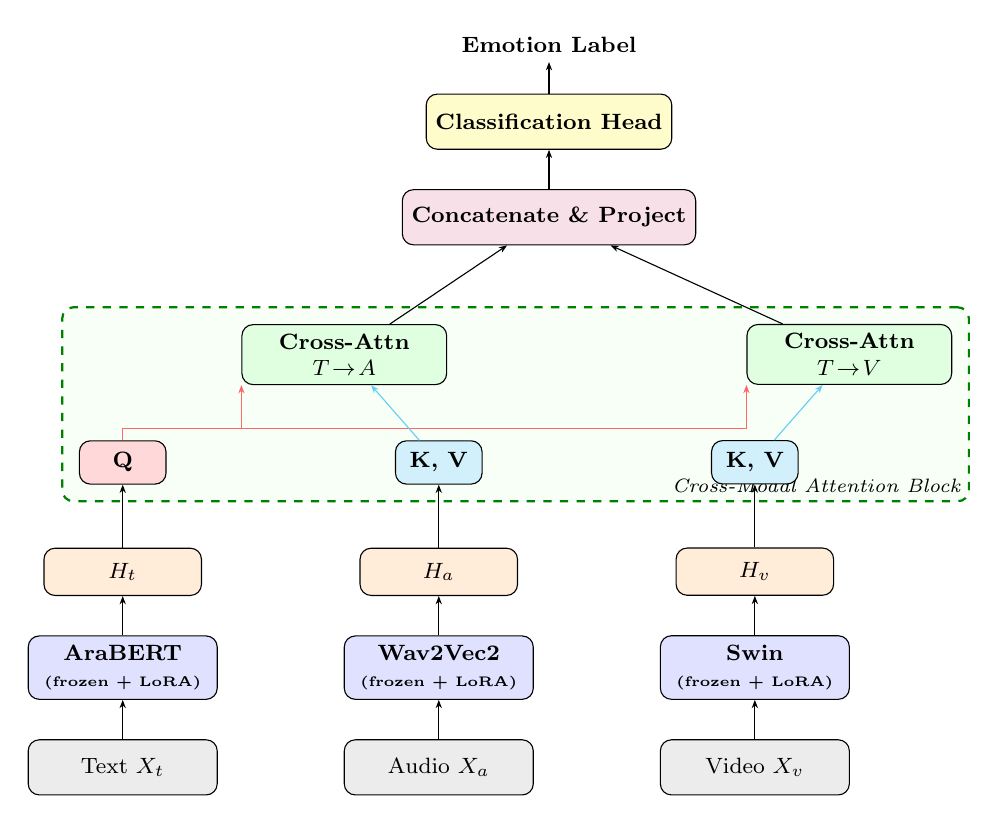
\begin{tikzpicture}[
    node distance=0.6cm and 0.8cm,
    >={Stealth[length=3pt]},
    encoder/.style={draw, rounded corners, fill=blue!12, minimum width=2.4cm, minimum height=0.7cm, font=\footnotesize\bfseries, align=center},
    feat/.style={draw, rounded corners, fill=orange!15, minimum width=2.0cm, minimum height=0.6cm, font=\footnotesize, align=center},
    qkv/.style={draw, rounded corners, minimum width=1.1cm, minimum height=0.55cm, font=\footnotesize\bfseries, align=center},
    attnblock/.style={draw, rounded corners, fill=green!12, minimum width=2.6cm, minimum height=0.7cm, font=\footnotesize\bfseries, align=center},
    fusebox/.style={draw, rounded corners, fill=purple!12, minimum width=3.0cm, minimum height=0.7cm, font=\footnotesize\bfseries, align=center},
    inputbox/.style={draw, rounded corners, fill=gray!15, minimum width=2.4cm, minimum height=0.7cm, font=\footnotesize, align=center},
    every edge/.style={draw, ->, thick},
]

% --- Input Layer ---
\node[inputbox] (text_in) {Text $X_t$};
\node[inputbox, right=1.6cm of text_in] (audio_in) {Audio $X_a$};
\node[inputbox, right=1.6cm of audio_in] (video_in) {Video $X_v$};

% --- Encoders ---
\node[encoder, above=0.5cm of text_in] (arabert) {AraBERT\\{\tiny (frozen + LoRA)}};
\node[encoder, above=0.5cm of audio_in] (wav2vec) {Wav2Vec2\\{\tiny (frozen + LoRA)}};
\node[encoder, above=0.5cm of video_in] (swin) {Swin\\{\tiny (frozen + LoRA)}};

% --- Feature Representations ---
\node[feat, above=0.5cm of arabert] (ht) {$H_t$};
\node[feat, above=0.5cm of wav2vec] (ha) {$H_a$};
\node[feat, above=0.5cm of swin] (hv) {$H_v$};

% --- Q, K, V labels ---
\node[qkv, fill=red!15, above=0.8cm of ht] (Q) {Q};
\node[qkv, fill=cyan!18, above=0.8cm of ha] (K) {K, V};
\node[qkv, fill=cyan!18, above=0.8cm of hv] (K2) {K, V};

% --- Cross-Attention Blocks ---
\node[attnblock, above=0.7cm of K, xshift=-1.2cm] (cma_ta) {Cross-Attn\\$T \!\rightarrow\! A$};
\node[attnblock, above=0.7cm of K2, xshift=1.2cm] (cma_tv) {Cross-Attn\\$T \!\rightarrow\! V$};

% --- Fusion ---
\node[fusebox, above=1.0cm of cma_ta, xshift=2.6cm] (fuse) {Concatenate \& Project};

% --- Output ---
\node[draw, rounded corners, fill=yellow!20, minimum width=2.6cm, minimum height=0.7cm, font=\footnotesize\bfseries, above=0.5cm of fuse] (cls) {Classification Head};
\node[above=0.4cm of cls, font=\footnotesize\bfseries] (out) {Emotion Label};

% --- Arrows: Input -> Encoder ---
\draw[->] (text_in) -- (arabert);
\draw[->] (audio_in) -- (wav2vec);
\draw[->] (video_in) -- (swin);

% --- Arrows: Encoder -> Features ---
\draw[->] (arabert) -- (ht);
\draw[->] (wav2vec) -- (ha);
\draw[->] (swin) -- (hv);

% --- Arrows: Features -> Q/K/V ---
\draw[->] (ht) -- (Q);
\draw[->] (ha) -- (K);
\draw[->] (hv) -- (K2);

% --- Arrows: Q/K/V -> Cross-Attention ---
\draw[->, color=red!60] (Q.north) -- ++(0, 0.15) -| (cma_ta.south west);
\draw[->, color=red!60] (Q.north) -- ++(0, 0.15) -| (cma_tv.south west);
\draw[->, color=cyan!60] (K) -- (cma_ta);
\draw[->, color=cyan!60] (K2) -- (cma_tv);

% --- Arrows: Cross-Attention -> Fusion ---
\draw[->] (cma_ta) -- (fuse);
\draw[->] (cma_tv) -- (fuse);

% --- Arrow: Fusion -> Classifier ---
\draw[->] (fuse) -- (cls);
\draw[->] (cls) -- (out);

% --- Background box around cross-attention ---
\begin{scope}[on background layer]
    \node[draw=green!50!black, dashed, thick, rounded corners, fill=green!3,
          fit=(Q)(K)(K2)(cma_ta)(cma_tv),
          inner sep=6pt, label={[font=\scriptsize\itshape, anchor=south east]south east:Cross-Modal Attention Block}] {};
\end{scope}

\end{tikzpicture}
\caption{Architecture of the proposed Tri-Modal Cross-Attention Network (Tri-CAN). Text features ($H_t$) serve as Queries (\textcolor{red}{Q}), while Audio ($H_a$) and Visual ($H_v$) features serve as Keys and Values (\textcolor{cyan!70!black}{K, V}). LoRA adapters are injected into each frozen encoder to enable parameter-efficient fine-tuning.}
\label{fig:trican}
\end{figure}

\subsection{Feature Extraction and Encoding}
To ensure a fair comparison with the EGY-MER benchmarks \citep{Hussein2025}, we utilize the same pre-trained encoders:
\begin{itemize}
    \item \textbf{Text ($X_t$):} We employ \textit{AraBERTv2-base}, a BERT-based model pre-trained on large-scale Arabic corpora, capable of handling dialectal nuances. The output is a sequence of hidden states $H_t \in \mathbb{R}^{L_t \times d_t}$.
    \item \textbf{Audio ($X_a$):} We utilize \textit{Wav2Vec2-Large-XLS-R}, extracting frame-level acoustic features $H_a \in \mathbb{R}^{L_a \times d_a}$ that capture pitch and intensity---critical indicators of sarcasm \citep{Hussien2018}.
    \item \textbf{Visual ($X_v$):} We use the \textit{Swin Transformer} to extract spatiotemporal features $H_v \in \mathbb{R}^{L_v \times d_v}$ from video frames, capturing facial action units (AUs) associated with emotional expression \citep{Hussein2025}.
\end{itemize}

\subsection{Cross-Modal Attention Mechanism}
The core innovation of our approach is the replacement of simple concatenation with a Scaled Dot-Product Attention mechanism. Given the dominance of text in sentiment analysis \citep{Alqarafi2019}, we use the text features ($H_t$) as the \textbf{Query ($Q$)}, while audio ($H_a$) and visual ($H_v$) features serve as \textbf{Keys ($K$)} and \textbf{Values ($V$)}.

For the Text-Audio interaction, the cross-modal attention is calculated as:
\begin{equation}
    \text{Attention}(Q, K, V) = \text{softmax}\left(\frac{H_t W_Q (H_a W_K)^T}{\sqrt{d_k}}\right) (H_a W_V)
\end{equation}

This mechanism allows the model to ``attend'' to specific spikes in audio energy (e.g., a shout) or specific visual frames (e.g., an eye-roll) that correspond to specific words, solving the alignment problem inherent in asynchronous multimodal data \citep{Haouhat2023}. This text-driven attention is applied to both non-verbal modalities ($T\rightarrow A$ and $T\rightarrow V$), producing text-guided audio and visual representations respectively, as illustrated in Figure~\ref{fig:trican}.

\paragraph{Relation to prior text-anchored architectures.} Using the textual stream as the anchoring modality is not itself novel, and the contribution claimed here should be stated precisely. \citet{Wang2022} motivate sparse cross-attention by the observation that text carries higher-order semantic content than audio or video; \citet{arXiv230713205v1} reinforce the non-verbal modalities under textual guidance for unaligned sequences; and \citet{Su2025} refine non-textual features hierarchically under text supervision. \citet{Yang2024} likewise learn tri-modal representations combining contrastive learning with a transformer, and should not be confused with the present architecture despite the similarity of name. Within Arabic specifically, \citet{Cheikhi2026} combine cross-modal attention with gated fusion.

The architectural contribution of Tri-CAN over these is accordingly modest and is not the basis of this proposal. What distinguishes the present work is the \emph{regime} in which the mechanism is evaluated: seven-class categorical emotion rather than three-class polarity, on a dialectal corpus roughly twenty-four times smaller than Ar-MuSA, with minority classes below 4\%. The relevant question is empirical rather than architectural---whether the advantage attention holds over late fusion in the sentiment setting persists when data are scarce and the decision is finer---and Section~\ref{sec:experiments} is designed to answer it in a form that is informative whichever way the result falls.

\subsection{Parameter-Efficient Fine-Tuning (PEFT)}
Training the full Tri-CAN architecture on the small EGY-MER dataset (363 samples) risks catastrophic overfitting. To mitigate this, we integrate \textbf{Low-Rank Adaptation (LoRA)}. Rather than updating all pre-trained weights $W$, we inject rank-decomposition matrices $A$ and $B$ into the attention layers:
\begin{equation}
    W' = W + \Delta W = W + BA
\end{equation}
Where $B \in \mathbb{R}^{d \times r}$ and $A \in \mathbb{R}^{r \times k}$, with rank $r \ll d$. This technique has been shown to reduce trainable parameters by up to 98\% while maintaining performance on Arabic tasks \citep{KhaledUniText2025}, making the architecture feasible for standard GPU hardware.

\subsection{Loss Function and Optimization}
Given the severe class imbalance in EGY-MER (where ``Fear'' and ``Surprise'' constitute $<4\%$ of data), standard Cross-Entropy Loss favors majority classes \citep{Hussein2025}. \textbf{Focal Loss} is employed, which applies a modulating factor $(1 - p_t)^\gamma$ to the loss, down-weighting easy examples and focusing training on hard, misclassified negatives:
\begin{equation}
    FL(p_t) = -\alpha_t (1 - p_t)^\gamma \log(p_t)
\end{equation}
We set $\gamma = 2$ and define $\alpha_t$ as the inverse class frequency, computed as $\alpha_t = N / (C \cdot N_t)$, where $N$ is the total number of samples, $C$ is the number of classes, and $N_t$ is the number of samples in class $t$. This ensures that rare emotions such as Fear and Surprise receive proportionally higher weight during training, counteracting the dominance of majority classes like Neutral.

% ----------------------------------------------------------------------

\section{Experimental Setup and Evaluation}\label{sec:experiments}

\subsection{Datasets}
Because the central question concerns whether a result transfers across task regimes, a single corpus cannot answer it. Three are therefore used, each with a distinct role:

\begin{itemize}
    \item \textbf{Target: EGY-MER} \citep{Hussein2025}. 363 single-speaker segments from Egyptian talk shows and dramas, annotated for seven emotions with severe class imbalance. This is the setting of interest and the corpus on which the 0.519 weighted F1 baseline stands.
    \item \textbf{Scale and dialect control: MORAD} \citep{Atou2026}. 2{,}325 unscripted videos from 329 speakers in Moroccan Arabic, annotated with the \emph{same} seven-emotion taxonomy as EGY-MER but roughly six times larger. Holding the label space fixed while varying corpus size and dialect separates two explanations for any observed difficulty that a single-corpus study necessarily conflates.
    \item \textbf{Calibration: Ar-MuSA} \citep{Khaled2025}. 8{,}700 samples annotated for three-class sentiment. Its role is methodological rather than substantive: because published results exist on this corpus \citep{Cheikhi2026, Cheikhi2026a, Cheikhi2026b}, an implementation that reproduces performance in that range provides external evidence that the architecture is correctly implemented. Without such an anchor, a result on EGY-MER---where no comparison point exists beyond the dataset's own baseline---would be difficult to falsify.
\end{itemize}

No model is trained across corpora, since the label spaces are incompatible. Each is trained and evaluated independently, and only the \emph{relative} margin between fusion strategies is compared across them. Absolute scores are not comparable between the sentiment and emotion settings and are not presented as such.

\subsection{Baselines}
Tri-CAN is compared against the following benchmarks:
\begin{enumerate}
    \item \textbf{Unimodal Baselines:} AraBERT (text only), Wav2Vec2 (audio only), and Swin (video only) \citep{Hussein2025}.
    \item \textbf{Gated Late Fusion:} The published EGY-MER baseline (weighted F1 0.519), which concatenates modality vectors at the classification stage \citep{Hussein2025}. This is the primary comparison, and---critically---it is re-implemented over the identical cached features used by Tri-CAN, so that the fusion mechanism is the only difference between the two conditions.
    \item \textbf{UniTextFusion:} A generative approach converting audio and video into textual descriptions for LLaMA-based classification \citep{KhaledUniText2025}.
    \item \textbf{Published Arabic attention-based results:} On Ar-MuSA only, the reported figures of \citet{Cheikhi2026}, \citet{Cheikhi2026a} and \citet{Cheikhi2026b} serve as external calibration.
\end{enumerate}

\subsection{Ablation Studies}
The following ablations test whether cross-modal attention contributes beyond simpler alternatives:
\begin{enumerate}
    \item \textbf{Bimodal Combinations:} (Text+Audio) against (Text+Video), to determine which non-verbal modality contributes most to Egyptian emotion recognition. Audio is hypothesised to dominate, given the tonal expressiveness of the dialect.
    \item \textbf{Fusion Mechanism:} Cross-modal attention against gated late fusion over identical features---the central comparison, repeated on all three corpora.
    \item \textbf{Attention Direction:} Text-as-query against symmetric bidirectional attention, testing whether the text-anchored asymmetry assumed in Section~\ref{sec:methodology} is warranted for emotion, where non-verbal cues carry proportionally more of the signal than they do for polarity.
    \item \textbf{Parameter-Efficient Adaptation:} Where compute permits, LoRA ranks $r \in \{4, 8, 16\}$ applied to the encoders. This is reported as a supplementary result rather than part of the main comparison, for the reason given in Section~\ref{sec:feasibility}.
\end{enumerate}

\subsection{Evaluation Protocol and Metrics}
Given the small size of EGY-MER (363 samples), a single train/test split would yield high-variance performance estimates. We therefore adopt \textbf{stratified 5-fold cross-validation}, ensuring that the class distribution---particularly for minority classes (Fear, Surprise)---is preserved in each fold. All reported metrics are averaged across folds with standard deviations to provide reliable comparisons.

Following the protocols in \citet{Hussein2025} and \citet{Rahma2023}, we report the following metrics:
\begin{itemize}
    \item \textbf{Weighted F1-Score:} The primary metric for overall performance, accounting for class imbalance.
    \item \textbf{Macro F1-Score:} To specifically evaluate the model's ability to detect minority classes (Fear, Surprise) without bias toward the majority class (Neutral).
    \item \textbf{Confusion Matrices:} Visualizing misclassifications to identify specific emotion pairs that are confused (e.g., Anger vs.\ Disgust).
    \item \textbf{Sarcasm Sensitivity:} A qualitative analysis of ``incongruent'' samples (where text polarity differs from ground truth emotion) to test the hypothesis that Cross-Attention better captures sarcasm.
\end{itemize}

\subsection{Feasibility and Compute Protocol}\label{sec:feasibility}
All encoders (AraBERT, Wav2Vec2-XLS-R, Swin) are available with open pre-trained weights. The corpora are not uniformly so: EGY-MER is not distributed publicly and requires authorisation from its creators, which constitutes the principal risk to this plan. MORAD and Amd'SaEr \citep{Atou2026, Haouhat2025a} are identified as substitutes whose taxonomies permit the research question to be posed with minimal restatement.

The experiments are designed for \textbf{CPU-only execution with frozen encoders}. Features are extracted once per corpus and cached; only the fusion block and classification head are trained. At the scale of EGY-MER this reduces training to minutes and makes five-fold cross-validation inexpensive.

This is presented as a methodological choice rather than merely a concession to available hardware, because it strengthens the central comparison. With encoders frozen and features shared, the \emph{only} difference between the late-fusion baseline and Tri-CAN is the fusion mechanism itself, so any margin between them is attributable to that mechanism alone. Fine-tuning the encoders---as the original formulation of this proposal envisaged---would confound the change in fusion with a change in representation, and would make an observed improvement harder to attribute. The LoRA configuration described in Section~\ref{sec:methodology} is accordingly retained as a supplementary ablation, to be conducted on external compute if time permits, rather than as part of the main result.

A residual feasibility concern is Ar-MuSA: extracting features for 8{,}700 samples on CPU is substantially more costly than for the smaller corpora. Should this prove prohibitive, the calibration anchor can be established on a stratified subsample, since its purpose is to verify implementation correctness rather than to establish a competitive result.

% ----------------------------------------------------------------------

\section{Conclusion}\label{sec:conclusion}

This literature review establishes that while 2025 marked a watershed moment for Arabic multimodal resources with the release of EGY-MER and Ar-MuSA, the modeling techniques applied to them have advanced unevenly. Attention-based fusion reached Arabic sentiment analysis during 2026 \citep{Cheikhi2026, Cheikhi2026a}, but dialectal \emph{emotion} recognition remains served by static late-fusion baselines that assume modality independence---an assumption that fails to capture the dynamic interplay of text, audio, and visual cues essential for understanding the high-context, sarcastic nature of Egyptian Arabic.

Through a systematic analysis of the existing approaches---from rudimentary concatenation to generative textualization and, most recently, to gated cross-modal attention \citep{Cheikhi2026}---this review identifies four critical gaps: the independence assumption in late fusion, the sarcasm bottleneck caused by modality incongruence, the data efficiency challenge posed by small-scale dialectal datasets, and the untested status of cross-modal attention for Arabic \emph{emotion} recognition, where the label space is finer, the class distribution far more skewed, and the available data an order of magnitude smaller than in the sentiment corpora on which the 2026 results were obtained. To address these gaps, this paper proposes the \textbf{Tri-Modal Cross-Attention Network (Tri-CAN)}. The contribution claimed is empirical rather than architectural: text-anchored cross-modal attention is established practice, and the open question is whether its reported advantage over late fusion persists when the label space is finer, the class distribution far more skewed, and the training data an order of magnitude smaller. Evaluating the mechanism across three corpora that vary task regime, scale and dialect independently yields an informative outcome in either direction---either an improvement on a baseline that has stood unchallenged since release, or evidence that attention-based fusion is not data-efficient enough for corpora of this size, which would itself be useful to anyone building on EGY-MER. The work thereby addresses the ``in-the-wild'' challenges identified by \citet{Hussien2018} and \citet{Rahma2023} and the future directions indicated by the dataset creators \citep{Hussein2025}.

% ----------------------------------------------------------------------

% BIBLIOGRAPHY SETUP
\bibliographystyle{plainnat}
\bibliography{references}

\end{document}


% Notes / To-Dos
%
% ADDRESSED 2026-08-04:
%  [x] Title: 'Literature Review' -> 'Systematic Review'. The word is now earned:
%      Sec 2.1 documents a pre-registered protocol, 3 databases, 20 queries,
%      citation snowballing, and PRISMA-style counts (1322 retrieved, 111
%      screened, 68 included).
%  [x] Structure made systematic: Sec 2.1 Review Methodology added, with an
%      explicit limitations paragraph.
%  [x] Sections lengthened with the 2026 literature: new Sec 2.4.5 on Arabic
%      cross-modal attention; datasets section extended with the 2025-26 Arabic
%      corpora; multimodal Arabic sarcasm added to Sec 2.3.
%  [x] Course-specific framing removed (author block, abstract, conclusion);
%      'we will' promissory tense removed.
%  [x] Gap 4 rewritten: the 'no cross-modal attention for Arabic' claim was
%      FALSIFIED by GCMA-Net (IEEE Access 2026) and two companion papers.
%      Restated as a task-regime question (sentiment vs emotion).
%  [x] Experimental setup updated to the three-corpus design and the CPU-only
%      frozen-encoder protocol.
%
% OUTSTANDING:
%  [ ] EGY-MER access unresolved. If it fails, MORAD/Amd'SaEr are the substitutes
%      (see rp2/PLAN.md). The feasibility section states this honestly.
%  [x] Abstracts: all 68 included works now have an indexed abstract; the two
%      DOI-less theses were verified by hand and added to references.bib.
%  [ ] Full texts not yet assessed for all 68 included works.
%  [ ] Consider whether 'Tri-CAN' should be renamed to avoid confusion with
%      Tri-CLT (Yang et al. 2024).